%%%%%%%%%%%%%%%%%%%%%%%%%%%%%%%%%%%%%%%%%%%%%%%%%%%%%%%%%%%%%%%%%%%%%%%%%%%%%%%%%%%%
% Document data
%%%%%%%%%%%%%%%%%%%%%%%%%%%%%%%%%%%%%%%%%%%%%%%%%%%%%%%%%%%%%%%%%%%%%%%%%%%%%%%%%%%%
\documentclass[12pt]{report} %report allows for chapters
\renewcommand\thesection{\arabic{section}} % ignore the title number for sections
%%%%%%%%%%%%%%%%%%%%%%%%%%%%%%%%%%%%%%%%%%%%%%%%%%%%%%%%%%%%%%%%%%%%%%%%%%%%%%%%%%%%




%%%%%%%%%%%%%%%%%%%%%%%%%%%%%%%%%%%%%%%%%%%%%%%%%%%%%%%%%%%%%%%%%%%%%%%%%%%%%%%%%%%%
% Packages
%%%%%%%%%%%%%%%%%%%%%%%%%%%%%%%%%%%%%%%%%%%%%%%%%%%%%%%%%%%%%%%%%%%%%%%%%%%%%%%%%%%%
\usepackage{color, soul, xcolor} % Colored text and highlighting, respectively

%Tikz
\usepackage{tikz-cd} % For commutative diagrams
\usepackage{tikz-3dplot}
\RequirePackage{pgfplots}
\usetikzlibrary{shadows}
\usetikzlibrary{shapes}
\usetikzlibrary{decorations}
\usetikzlibrary{arrows,decorations.markings} 
\usetikzlibrary{quotes,angles}

\usepackage{mathtools}
\usepackage{answers}
\usepackage{setspace}
\usepackage{graphicx}
\usepackage{enumerate}
\usepackage{multicol}
\usepackage{mathrsfs}
\usepackage[margin=1in]{geometry} 
\usepackage{amsmath,amsthm,amssymb}
\usepackage{marvosym,wasysym} %fucking smileys
\usepackage{subcaption}
\usepackage{morefloats}
\usepackage{float}
\usepackage{hyperref}
%%%%%%%%%%%%%%%%%%%%%%%%%%%%%%%%%%%%%%%%%%%%%%%%%%%%%%%%%%%%%%%%%%%%%%%%%%%%%%%%%%%%




%%%%%%%%%%%%%%%%%%%%%%%%%%%%%%%%%%%%%%%%%%%%%%%%%%%%%%%%%%%%%%%%%%%%%%%%%%%%%%%%%%%%
% Shortcuts
%%%%%%%%%%%%%%%%%%%%%%%%%%%%%%%%%%%%%%%%%%%%%%%%%%%%%%%%%%%%%%%%%%%%%%%%%%%%%%%%%%%%
% Number systems
\newcommand{\N}{\mathbb{N}}
\newcommand{\Z}{\mathbb{Z}}
\newcommand{\C}{\mathbb{C}}
\newcommand{\R}{\mathbb{R}}
\newcommand{\Q}{\mathbb{Q}}
\newcommand{\partialx}{\frac{\partial f}{\partial x}}
\newcommand{\partialy}{\frac{\partial f}{\partial y}}
\newcommand{\partialz}{\frac{\partial f}{\partial z}}

% Operators/functions
\newcommand{\id}{\mathrm{Id}}
\newcommand{\RE}{\mathrm{Re}}
\newcommand{\IM}{\mathrm{Im}}
\DeclareMathOperator{\sech}{sech}
\DeclareMathOperator{\csch}{csch}
%%%%%%%%%%%%%%%%%%%%%%%%%%%%%%%%%%%%%%%%%%%%%%%%%%%%%%%%%%%%%%%%%%%%%%%%%%%%%%%%%%%%




%%%%%%%%%%%%%%%%%%%%%%%%%%%%%%%%%%%%%%%%%%%%%%%%%%%%%%%%%%%%%%%%%%%%%%%%%%%%%%%%%%%%
% Environments
%%%%%%%%%%%%%%%%%%%%%%%%%%%%%%%%%%%%%%%%%%%%%%%%%%%%%%%%%%%%%%%%%%%%%%%%%%%%%%%%%%%%
% Italic font
\newtheorem{theorem}{Theorem}[section]
\newtheorem{lemma}{Lemma}[section]
\newtheorem{corollary}{Corollary}[section]
\newtheorem{axiom}{Axiom}

% Plain font
\theoremstyle{definition}
\newtheorem{definition}{Definition}[section]
\newtheorem{example}{Example}[section]
\newtheorem{remark}{Remark}[section]
\newtheorem{solution}{Solution}
\newtheorem{problem}{Problem}[section]
\newtheorem{question}{Question}[section]
\newtheorem{answer}{Answer}[section]
\newtheorem{exercise}{Exercise}[section]
%%%%%%%%%%%%%%%%%%%%%%%%%%%%%%%%%%%%%%%%%%%%%%%%%%%%%%%%%%%%%%%%%%%%%%%%%%%%%%%%%%%%

\begin{document}


\begin{center}
   \textsc{\large MATH 255, Homework 4: \emph{Solutions}}\\
\end{center}
\vspace{.5cm}

\noindent\textbf{Relevant Sections:} 8.1, 8.2, 8.3, 8.4, 8.5, 8.6 \\

\noindent\textbf{Problem 1.} Evaluate the following expressions and simplify to the form $z=a+bi$.
\begin{enumerate}[(a)]
    \item Let $z_1=6+7i$ and $z_2=-3+3i$.  Find $z_1+z_2$ and $z_1-z_2$.
    \item Let $z_1=5+5i$ and $z_2=-1+2i$.  Find $z_1\cdot z_2$ and $z_1/z_2$.
    \item Take the complex number $z=i+1$ and multiply by $i$ until you return to your starting point.  This should take four iterations.
\end{enumerate}

\begin{solution}~
\begin{enumerate}[(a)]
    \item We have
    \begin{align*}
        z_1+z_2 = (6+7i)+(-3+3i)=(6-3)+i(7+3)=3+10i,
    \end{align*}
    and
    \begin{align*}
        z_1-z_2 = (6+7i)-(-3+3i)=(6-(-3))+i(7-3)=9+4i.
    \end{align*}
    \item We have
    \begin{align*}
        z_1\cdot z_2 = (5+5i)\cdot (-1+2i) = -5-5i+10i-10=-15+5i,
    \end{align*}
    and
    \begin{align*}
        z_1/z_2 = z_1 \cdot z_2^{-1} = (5+5i)\cdot \frac{1}{1^2+2^2}(-1-2i)=\frac{1}{5}(-5-5i-10i+10)=1-3i.
    \end{align*}
    \item Take
    \begin{align}
    i(i+1) &= -1+i\\    
    i(-1+i) &= -1-i\\
    i(-1-i) &= 1-i\\
    i(1-i) &= 1+i.
    \end{align}
\end{enumerate}
\end{solution}


\noindent\textbf{Problem 2.} Plot the following points in the complex plane $\C$.  Then for each point $z=a+bi$ rewrite in polar form $z=re^{i\theta}$. For each point given in polar form $z=r^{i\theta}$ rewrite it in cartesian form as $z=a+bi$ by using Euler's formula.
\begin{enumerate}[(a)]
    \item From your work on Problem 1 (c) plot and write in polar form the following:
    \begin{itemize}
        \item $z_1=i+1$.
        \item $z_2=i(i+1)$.
        \item $z_3=i^2(i+1)$.
        \item $z_4=i^3(i+1)$.
        \item $z_5=i^4(i+1)$.
    \end{itemize}
    \item $z_6=4-5i$.
    \item $z_7=3e^{i(\pi/2)}$.
    \item $z_8=2e^{i(5\pi/4)}$.
    \item $z_9=4e^{i(0)}$.
\end{enumerate}

\begin{solution}
Here is a plot for each point
        \begin{center}
        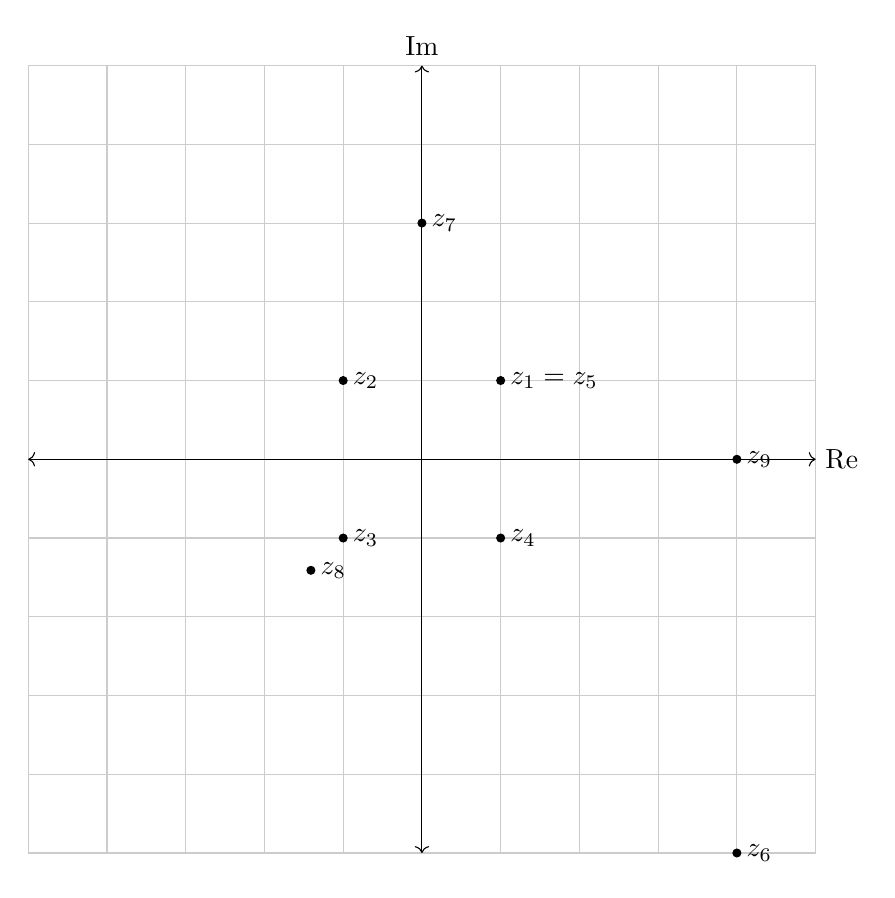
\begin{tikzpicture}
        \draw[thin,gray!40] (-5,-5) grid (5,5);
        \draw[<->] (-5,0)--(5,0) node[right]{$\RE$};
        \draw[<->] (0,-5)--(0,5) node[above]{$\IM$};
        \foreach \Point/\PointLabel in {(1,1)/{z_1=z_5}, (-1,1)/z_2, (-1,-1)/z_3, (1,-1)/z_4, (4,-5)/z_6, (0,3)/z_7, (-1.41,-1.41)/z_8, (4,0)/z_9}
        \draw[fill=black] \Point circle (0.05) node[right] {$\PointLabel$};
        \end{tikzpicture}
        \end{center}
        \begin{enumerate}[(a)]
            \item We have
            \begin{itemize}
                \item $z_1 = 1+i = \sqrt{2}e^{i(\pi/4)}$,
                \item $z_2 = -1+i = \sqrt{2}e^{i(3\pi/4)}$,
                \item $z_3 = -1-i = \sqrt{2}e^{i(5\pi/4)}$,
                \item $z_4 = 1-i = \sqrt{2}e^{i(7\pi/4)}$,
                \item $z_5 = 1+i = \sqrt{2}e^{i(9\pi/4)}=z_1$.
            \end{itemize}
            
            \item We have 
            \[
            r= \sqrt{4^2+5^2}=\sqrt{41},
            \]
            and
            \[
            \theta = \arctan \left( \frac{-5}{4}\right)\approx 0.896.
            \]
            So we can write
            \[
            z_6 = 4-5i = \sqrt{41}e^{0.896i}.
            \]
            \item If we want this number in cartesian form, $a+bi$, then we have 
            \[
            a=r\cos \theta = 3 \cos\left( \frac{\pi}{2}\right) = 0,
            \]
            and
            \[
            b = r \sin \theta = 3 \sin \left( \frac{\pi}{2}\right) = 3.
            \]
            So
            \[
            z_7 = 3e^{i(\pi/2)} = 0+3i.
            \]
            \item Similarly,
            \[
            a = 2\cos \left( \frac{5\pi}{4}\right) = -\sqrt{2},
            \]
            and
            \[
            b = 2 \sin \left(\frac{5\pi}{4}\right) = -\sqrt{2}.
            \]
            So
            \[
            z_8 = 2e^{i(5\pi/4)}.
            \]
            \item Note that $e^{i0}=e^0=1$ so 
            \[
            z_9 = 4e^{i(0)}=4.
            \]
        \end{enumerate}
\end{solution}

\noindent\textbf{Problem 3.} Complex functions (i.e., functions $f\colon \C \to \C$) are tricky to visualize.  The issue is that both the input and output are 2-dimensional which means you need some way to visualize 4-dimensional space.  For the following, I want you to visit \url{www.complexgrapher.com} and plot the following functions. Please print these out and attach them to your homework. 
\begin{enumerate}[(a)]
    \item $f\colon \C \to \C$ given by $f(z)=z$.
    \item $g\colon \C \to \C$ given by $g(z)=z^2$.
    \item $h\colon \C \to \C$ given by $h(z)=z^3$.
    \item $p\colon \C \to \C$ given by $p(z)=\sin z$.
    \item $q\colon \C \to \C$ given by $q(z)=\frac{1}{z^2+1}$.
\end{enumerate}
How does this plotting work?  Pick a point $z=a+ib$ on the plane as your input, and if you look at that point, the brightness of each pixel tells you the magnitude $r$ of each complex number and the hue tells you the argument (or angle, or phase) $\theta$ of the complex number. Try adjusting the \emph{magnitude modulus}.  Adjusting this will give you more of an idea as to what is happening.  For example, with the magnitude modulus set to $m$, you are seeing the remainder of the magnitude $r$ when you divide by $m$.  That is to say, for example, $1+m$ and $1$ will be shown with the same brightness.

\begin{solution}~
\begin{figure}[H]
    \centering
   \begin{subfigure}[h]{0.45\textwidth}
        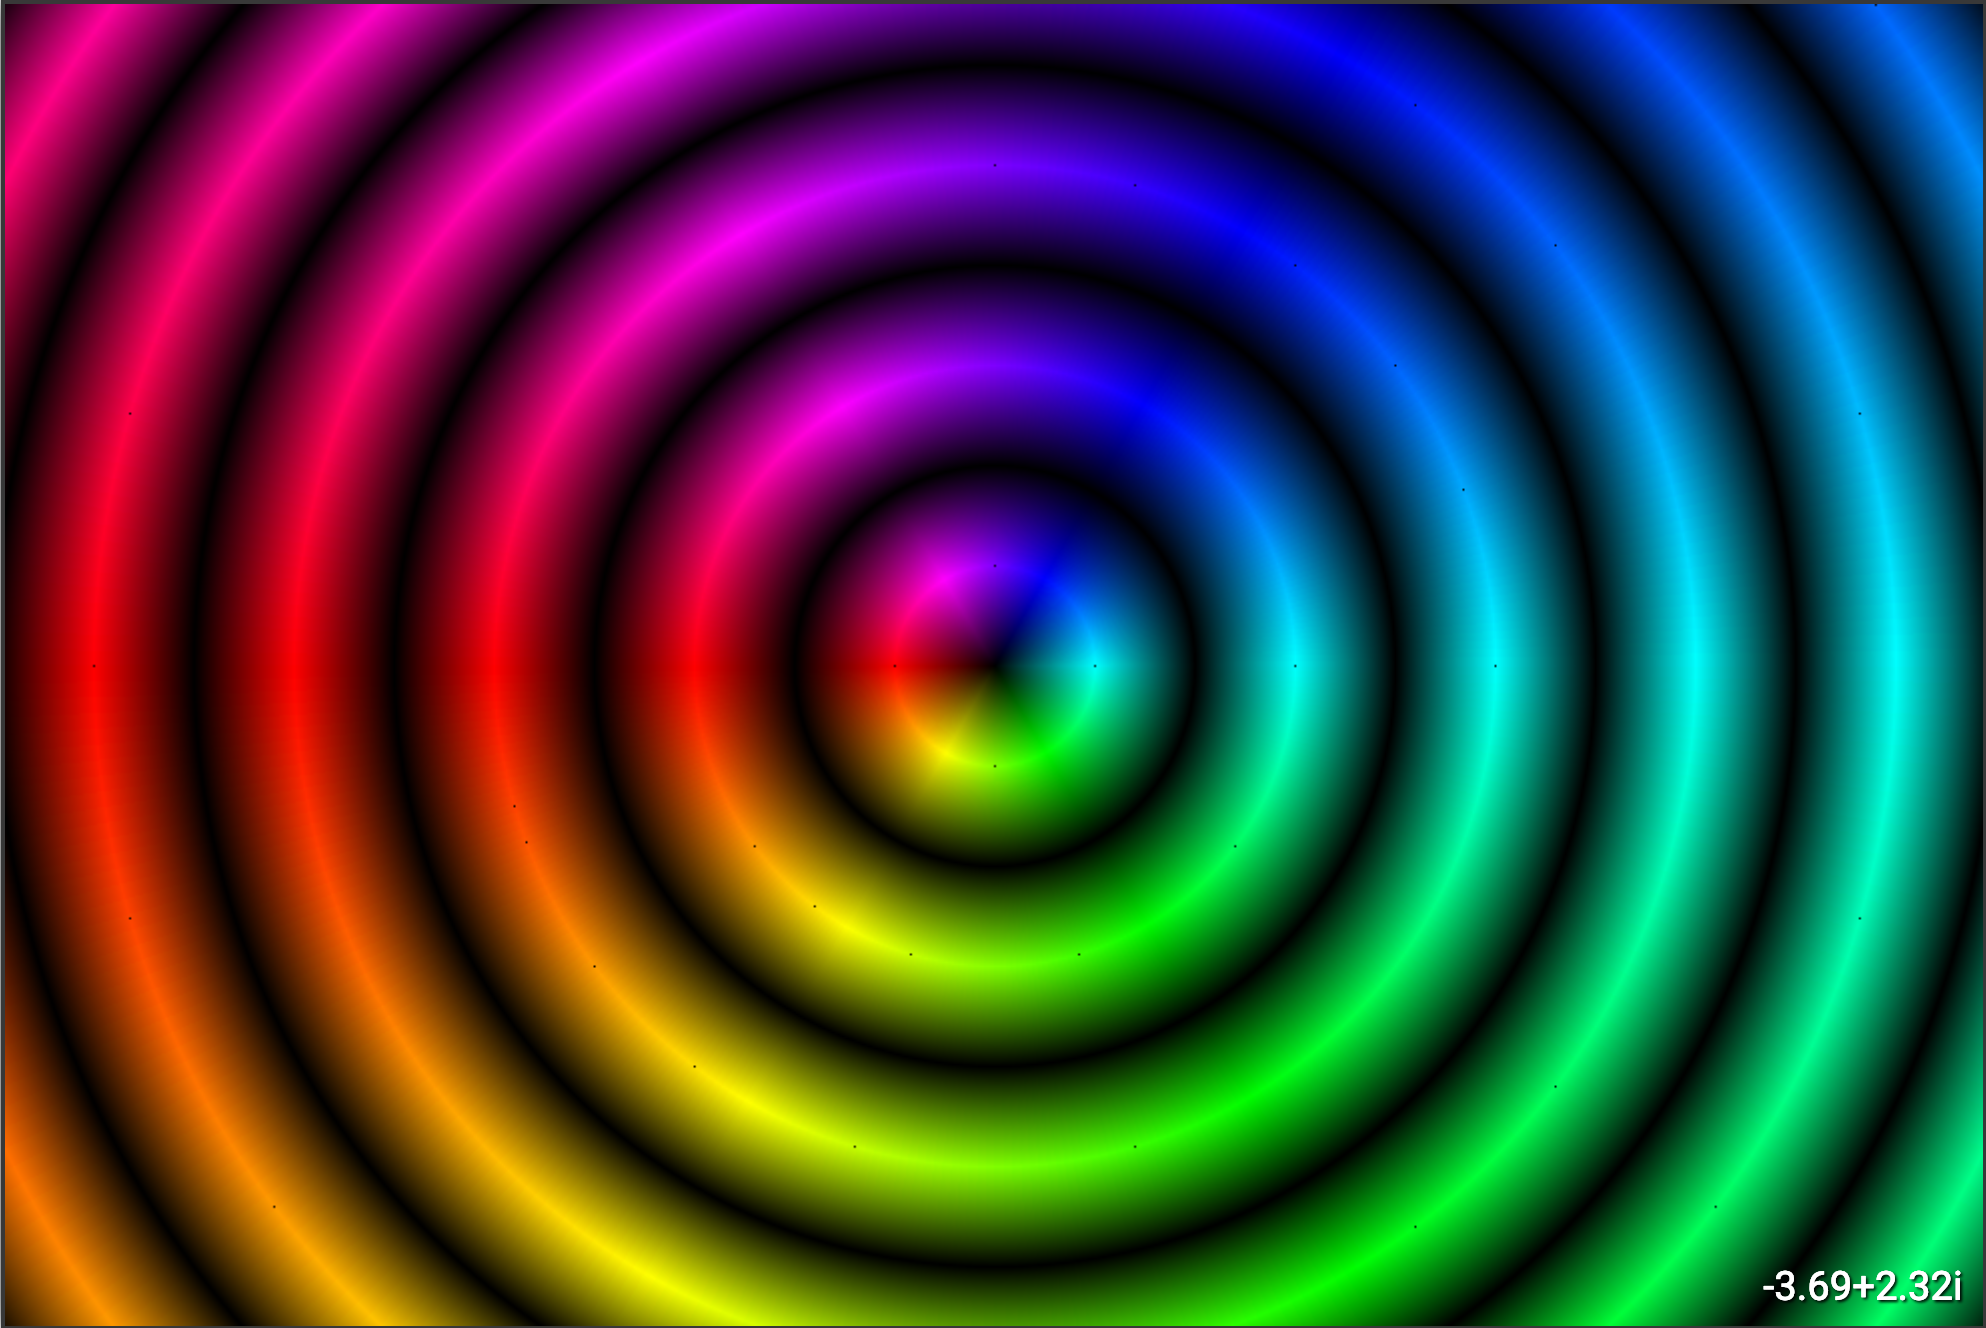
\includegraphics[width=\textwidth]{Images/z_plot.png}
        \caption{Plot of $f$.}
    \end{subfigure}
    ~ 
    \begin{subfigure}[h]{0.45\textwidth}
        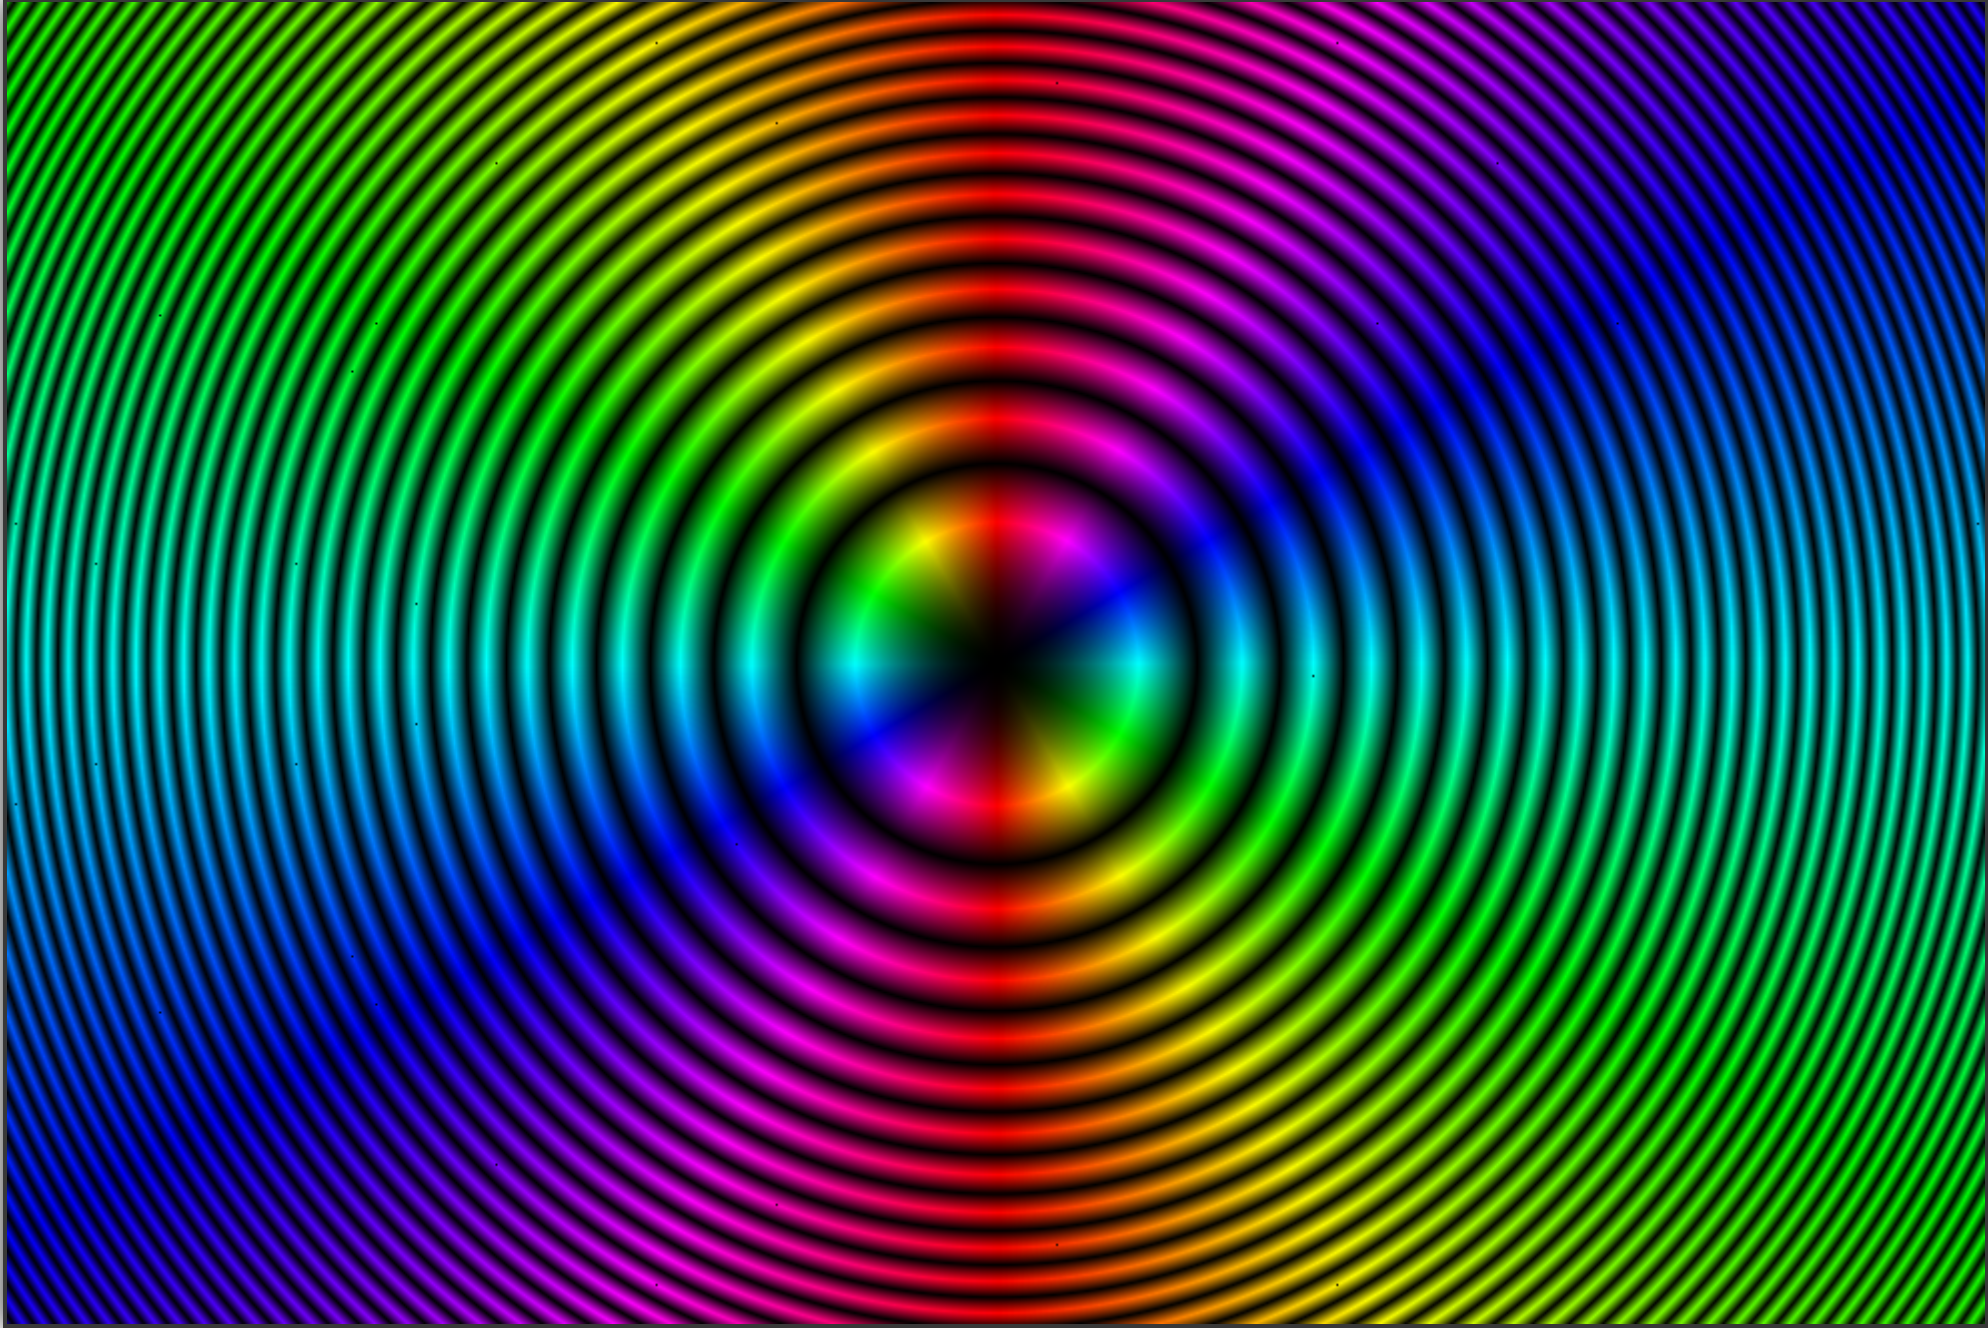
\includegraphics[width=\textwidth]{Images/z2_plot.png}
        \caption{Plot of $g$.}
    \end{subfigure}
    
    \begin{subfigure}[h]{0.45\textwidth}
        \includegraphics[width=\textwidth]{Images/z3_plot.png}
        \caption{Plot of $h$.}
    \end{subfigure}
    ~
    \begin{subfigure}[h]{0.45\textwidth}
        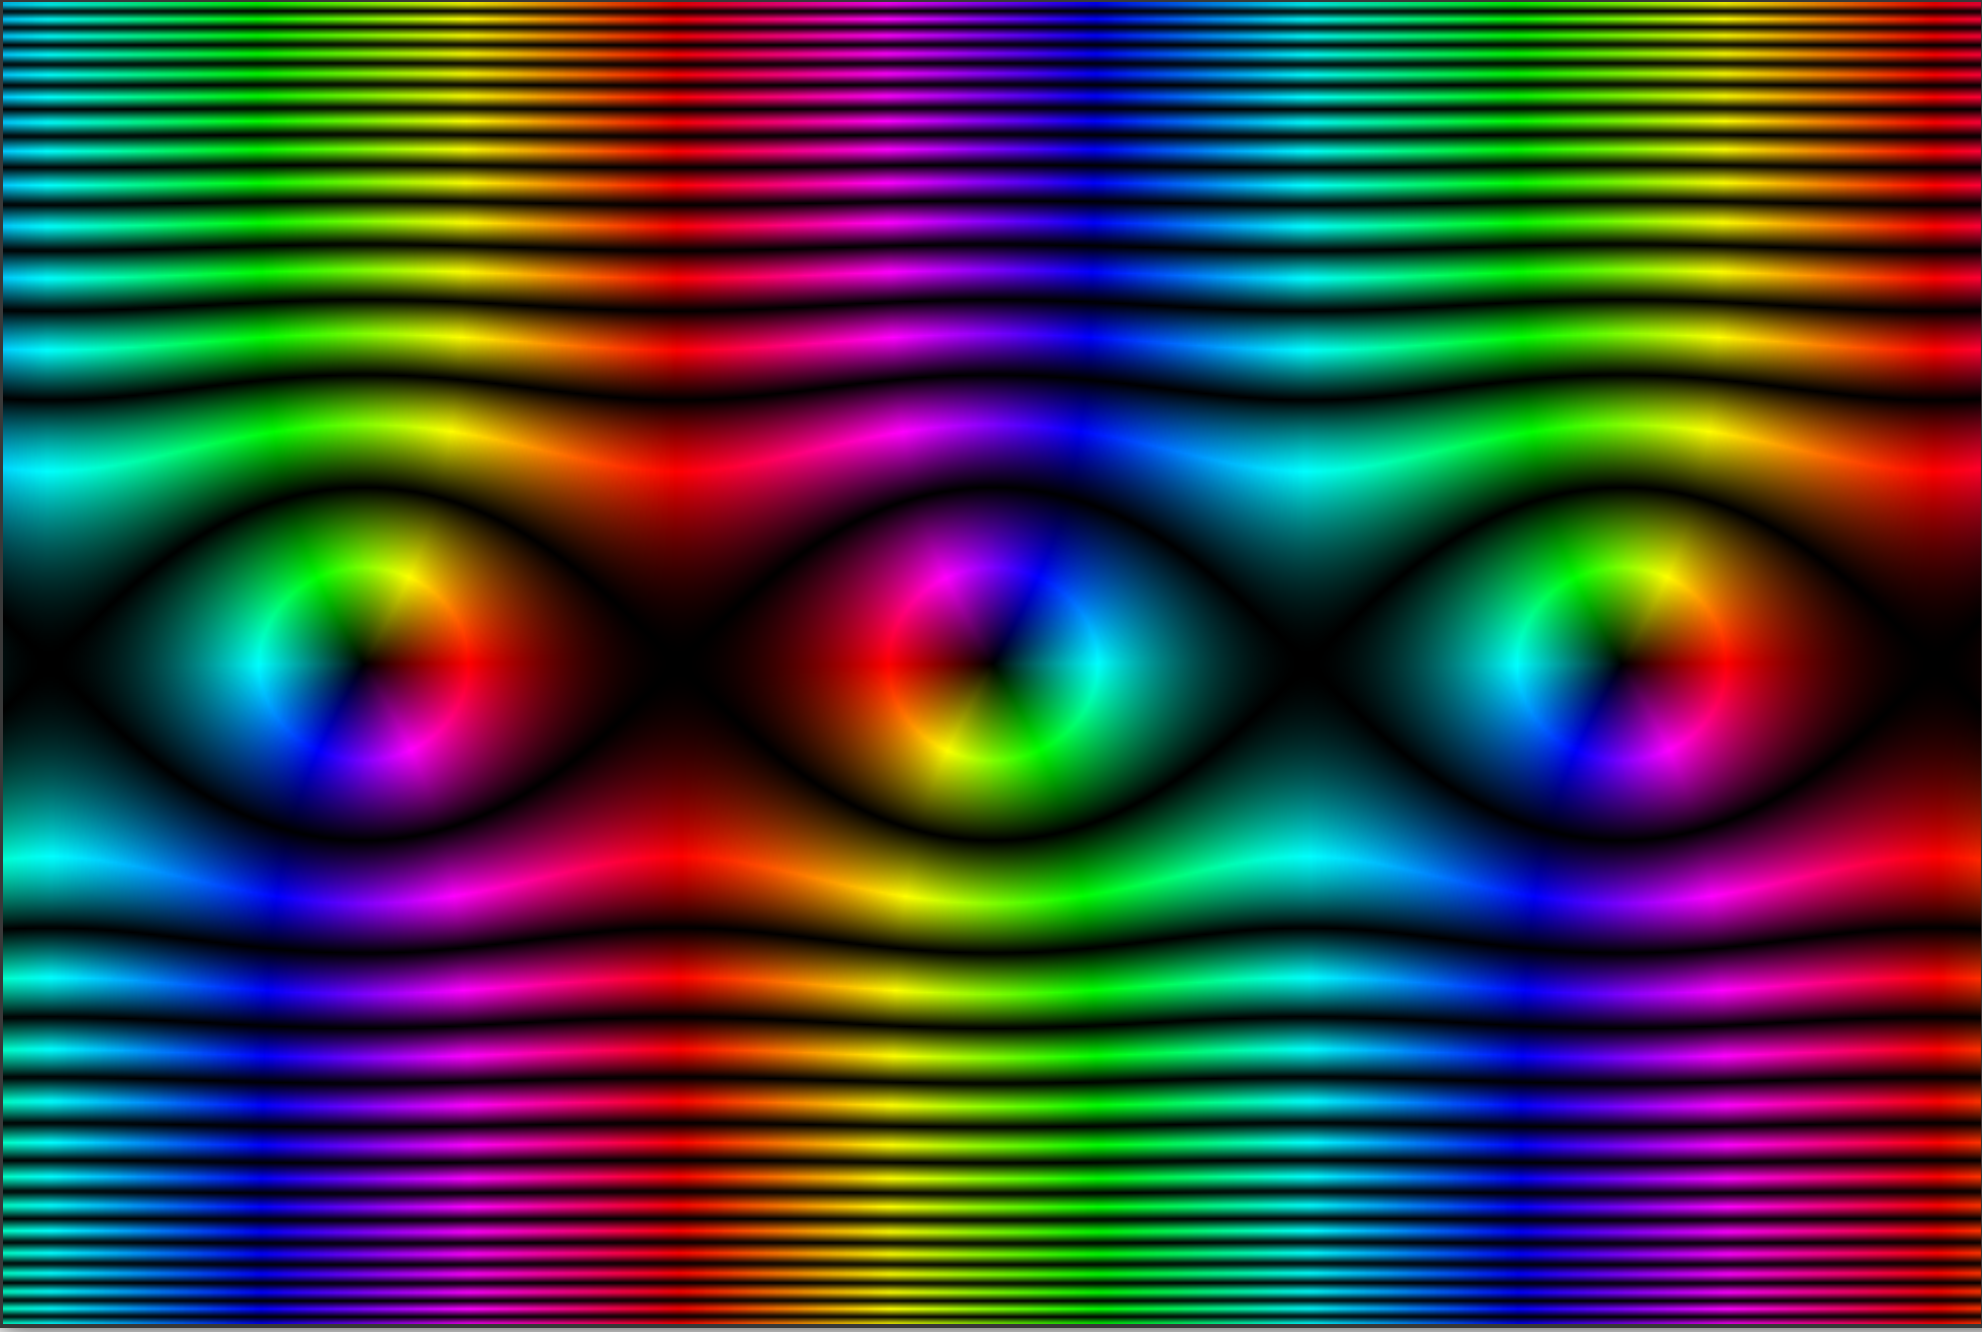
\includegraphics[width=\textwidth]{Images/sinz_plot.png}
        \caption{Plot of $p$.}
    \end{subfigure}
    
    \begin{subfigure}[h]{0.45\textwidth}
        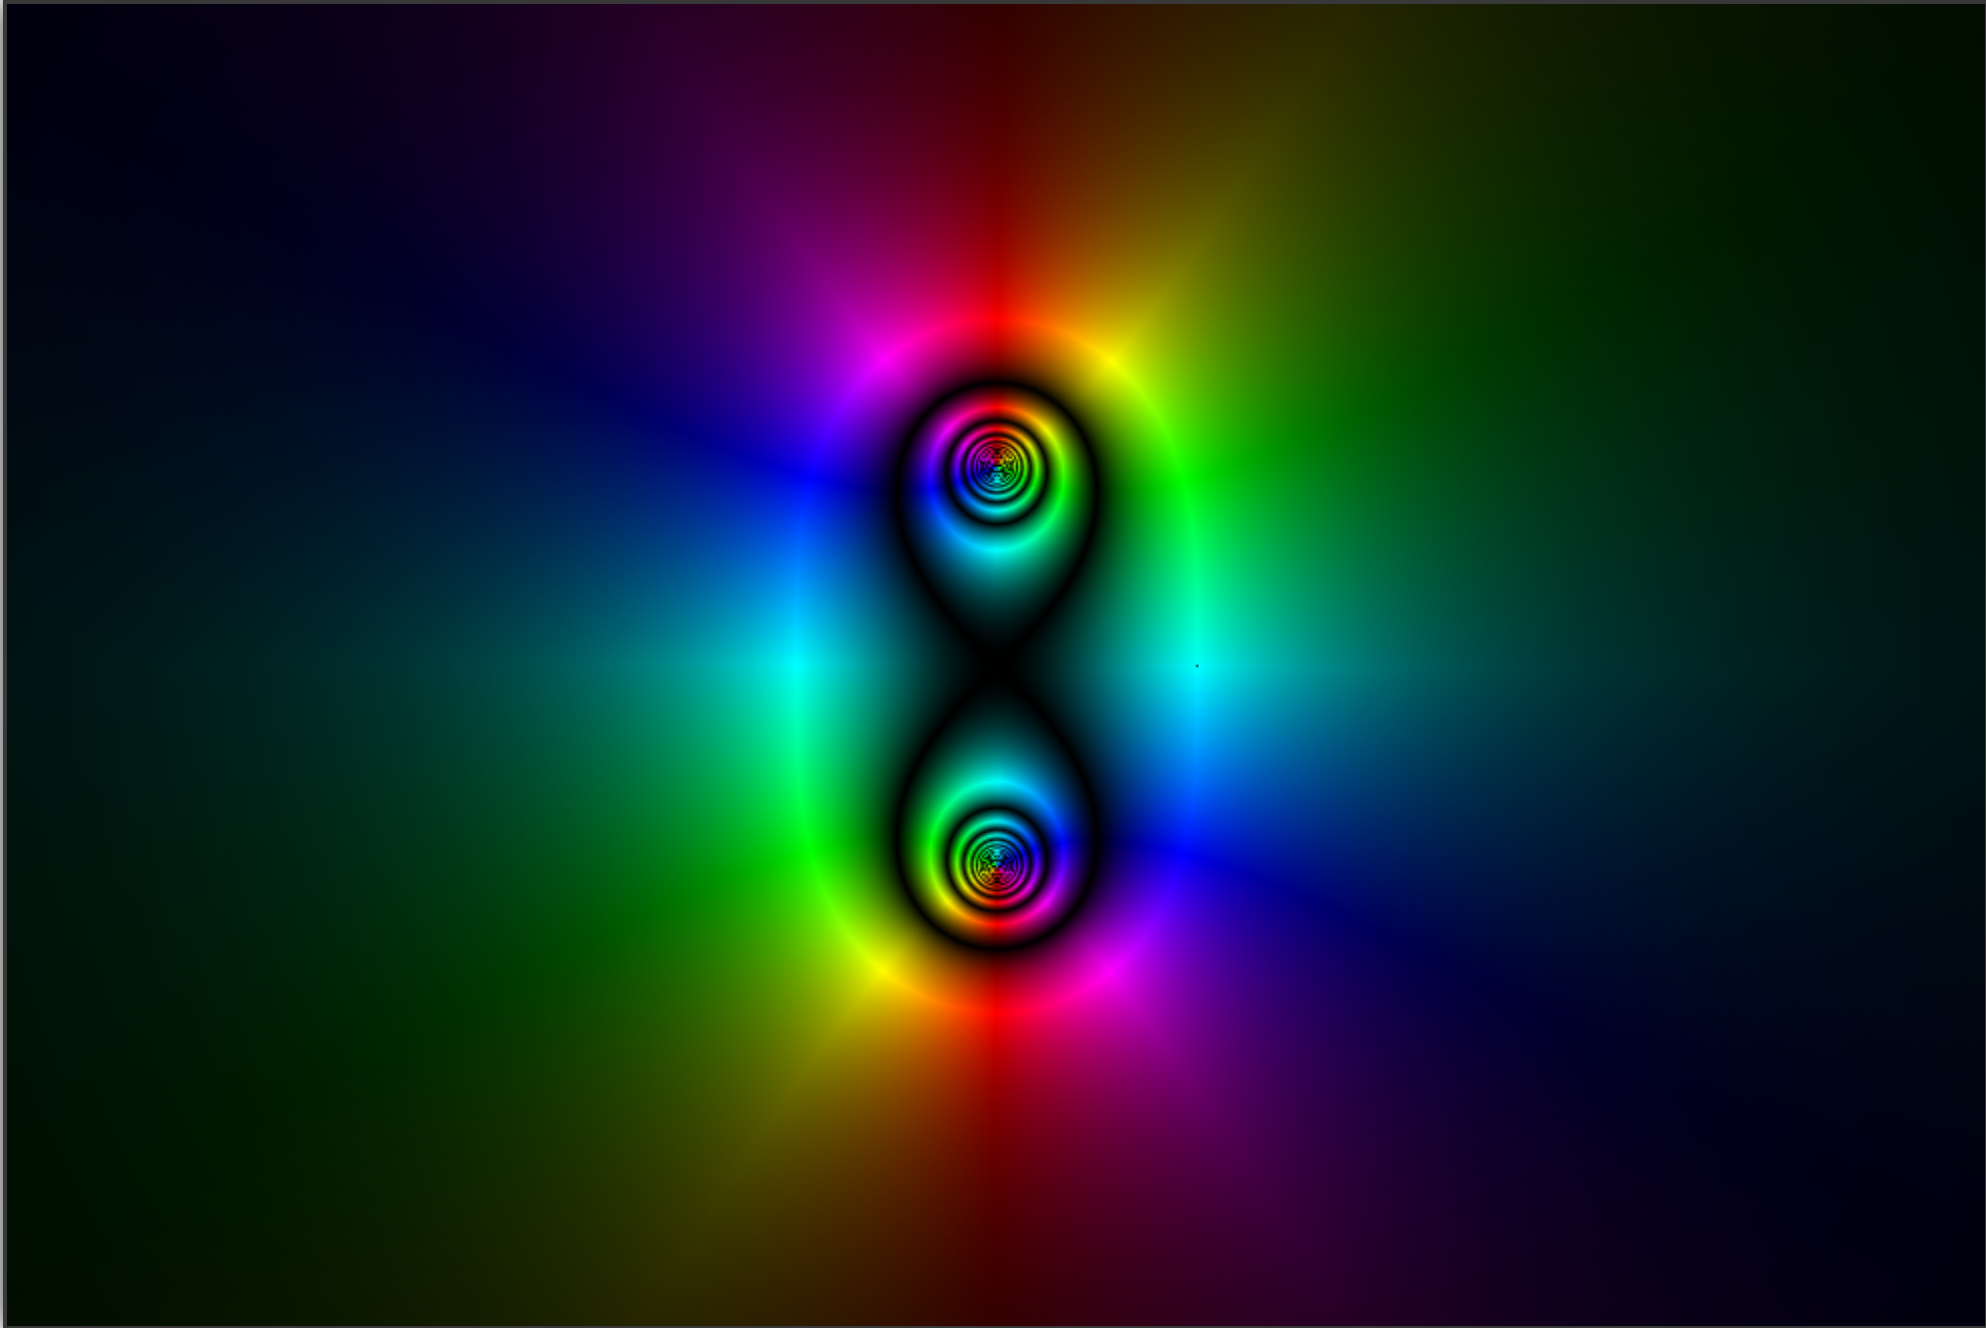
\includegraphics[width=\textwidth]{Images/rationalz_plot.png}
        \caption{Plot of $q$.}
    \end{subfigure}
\end{figure}
\end{solution}

\noindent\textbf{Problem 4.} The point of developing complex numbers is to give us the ability to factor any polynomial.  That is, a function of the form
\[
f(z)=a_0 + a_1 z + a_2 z^2 + \cdots + a_n z^n.
\]
By giving us the ability to find $\sqrt{-1}$, we can actually factor any polynomial.  Restated, the \emph{fundamental theorem of algebra} says that any polynomial of degree $n$ (the highest power of $z$ in your polynomial) with complex coefficients ($a_i \in \C$) has $n$ complex roots (zeros).  
For the following, find the roots of the polynomials using WolframAlpha when necessary.
\begin{enumerate}[(a)]
    \item $z^2+2$.
    \item $z^3+z^2+z+1$.
    \item $z^4+z^3+z^2+z+1$.
    \item $z^n-1$. These are commonly called the \emph{roots of unity}.
\end{enumerate}

\begin{solution}~
\begin{enumerate}[(a)]
    \item Here we can solve directly,
    \begin{align*}
        z^2+2&=0\\
        \implies z^2&=-2\\
        \implies z &= \pm i\sqrt{2}.
    \end{align*}
    \item Here, we can use WolframAlpha since the cubic formula is awful. We find that the roots are
    \[
    z= -1, ~ z=-i, ~ z=i.
    \]
    \item Similarly, the quartic formula is even worse, so we use WolframAlpha. We get
    \[
    z=-(-1)^{1/5}, ~z=(-1)^{2/5}, ~z=-(-1)^{3/5}, ~z=(-1)^{4/5}.
    \]
    But what do these even mean? We don't know what it means to take take these powers here.  
    \item Here, we can see a bit more about what these powers really mean by investigating a special case.  Namely, we want all the numbers whose $n$th power is $1$ since
    \begin{align*}
        z^n-1&=0\\
        \implies z^n = 1.
    \end{align*}
    The idea here is that all complex numbers of length 1 are merely just rotations.  So we want to break down the rotation of $2\pi$ into equal increments. See the picture below for $n=2$, $n=3$, and $n=4$
    \begin{figure}[H]
        \centering
        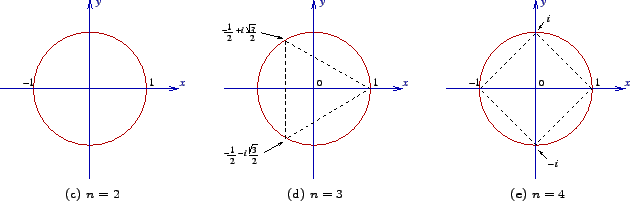
\includegraphics[width=\textwidth]{Images/roots_unity.png}
    \end{figure}
    This is the type of question that you should Google and try to read about in order to find the solution.  I'd argue that I didn't teach you quite enough for you to easily go about doing this, but you can spend the time to read some on this and see what is done.  See \url{https://en.wikipedia.org/wiki/Root_of_unity}.  Here is the solution, though:
    \[
    z = e^{\frac{i2\pi m}{n}} ~\textrm{for } m=0,1,2, \dots, n-1. 
    \]
\end{enumerate}
\end{solution}

\noindent\textbf{Problem 5.} We ran into an issue previously with finding eigenvalues for the following matrix:
\[
A=\begin{bmatrix} 0 & -1 \\ 1 & 0 \end{bmatrix}.
\]
Now we have the tools to solve this.  Show that the eigenvalues are $\pm i$ and that the corresponding eigenvectors are 
\[
\mathbf{v}_1 = \begin{bmatrix} i \\ 1 \end{bmatrix} \qquad \mathbf{v}_2 = \begin{bmatrix} -i \\ 1 \end{bmatrix}.
\]
Recall that this matrix was one that rotates vectors in the plane by $\pi/2=90^\circ$.  The remarkable fact is that the eigenvalues being $\pm i$ capture this same phenomenon.  If you look at what happens in Problem 1 and 2 you can see that multiplication of a complex number by $i$ acts like rotation of a vector in the plane.

\begin{solution}
To find the eigenvalues, we solve
\[
\det(A-\lambda I) = 0.
\]
So, we get
\[
A-\lambda I = \begin{bmatrix} -\lambda & -1 \\ 1 & -\lambda \end{bmatrix}.
\]
Then 
\[
\det(A-\lambda I) = \lambda^2 + 1 = 0
\]
has solutions $\lambda_1 = i$ and $\lambda_2 = -i$.\\

\noindent \underline{For $\lambda_1$:}
We find the eigenvectors by
\[
(A-iI)\mathbf{v}_1 = \mathbf{0}
\]
Which we can make into an augmented matrix
\[
    M=\left[ \begin{array}{cc|c}
        -i & -1 & 0\\
        1 & -i & 0
    \end{array}\right].
\]
Notice $R2$ is $i$ times $R1$ (things are a bit more complicated since we can use complex numbers now), so we have
\[
    M=\left[ \begin{array}{cc|c}
        -i & -1 & 0\\
        0 & 0 & 0
    \end{array}\right],
\]
which letting the $y=1$, gives us $x=i$. So
\[
\mathbf{v}_1 = \begin{bmatrix} i\\ 1 \end{bmatrix}.
\]

\noindent \underline{For $\lambda_2$:}
We find the eigenvectors by
\[
(A+iI)\mathbf{v}_2 = \mathbf{0}
\]
Which we can make into an augmented matrix
\[
    M=\left[ \begin{array}{cc|c}
        i & -1 & 0\\
        1 & i & 0
    \end{array}\right].
\]
Notice $R1$ is $i$ times $R2$ (things are a bit more complicated since we can use complex numbers now), so we have
\[
    M=\left[ \begin{array}{cc|c}
        0 & 0 & 0\\
        1 & i & 0
    \end{array}\right],
\]
which letting the $y=1$, gives us $x=-i$. So
\[
\mathbf{v}_2 = \begin{bmatrix} -i\\ 1 \end{bmatrix}.
\]
\end{solution}





\end{document}  